\chapter{Teoreticky rozbor}
bla bla bla
\section{\acl{DPS}}
\section{Hardver}
\subsection{snimac teploty}
\subsection{snimac tlaku}
\subsection{snimac vlhkosti}
\subsection{Raspberry PI}
Raspberry Pi je jednodoskový počítač s doskou veľkosti zhruba platobnej karty, prípadne ide o niečo menšiu doštičku (výpočtový modul). Vyvíja ho britská nadácia Raspberry Pi Foundantion s cieľom podporiť výučbu informatiky v školách.
\begin{figure}[h!]
    \centering
    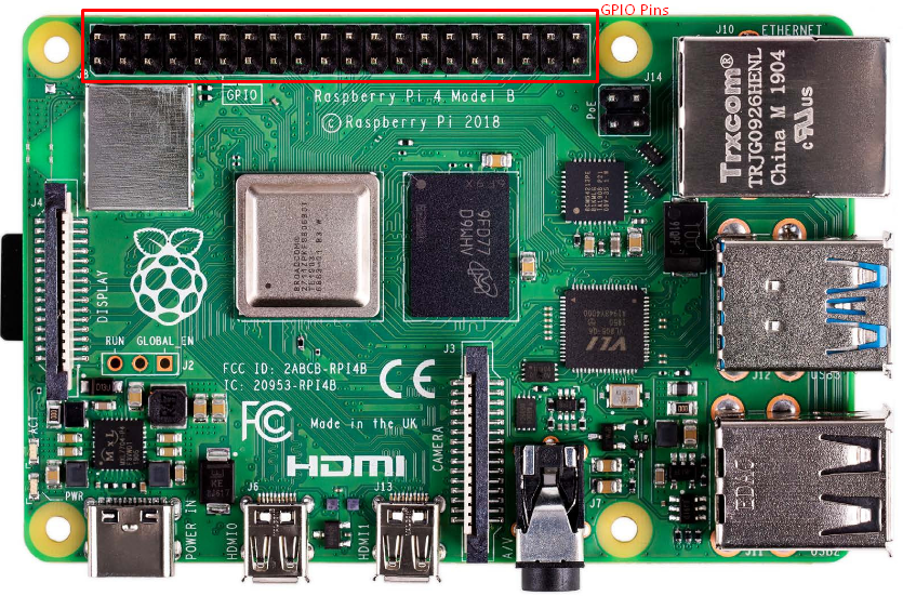
\includegraphics[width=0.4\textwidth]{obrazky/RPi.png}
    \caption{Raspberry PI 4}
\end{figure}
\subsubsection{GPIO header}
\begin{figure}[h!]
    \centering
    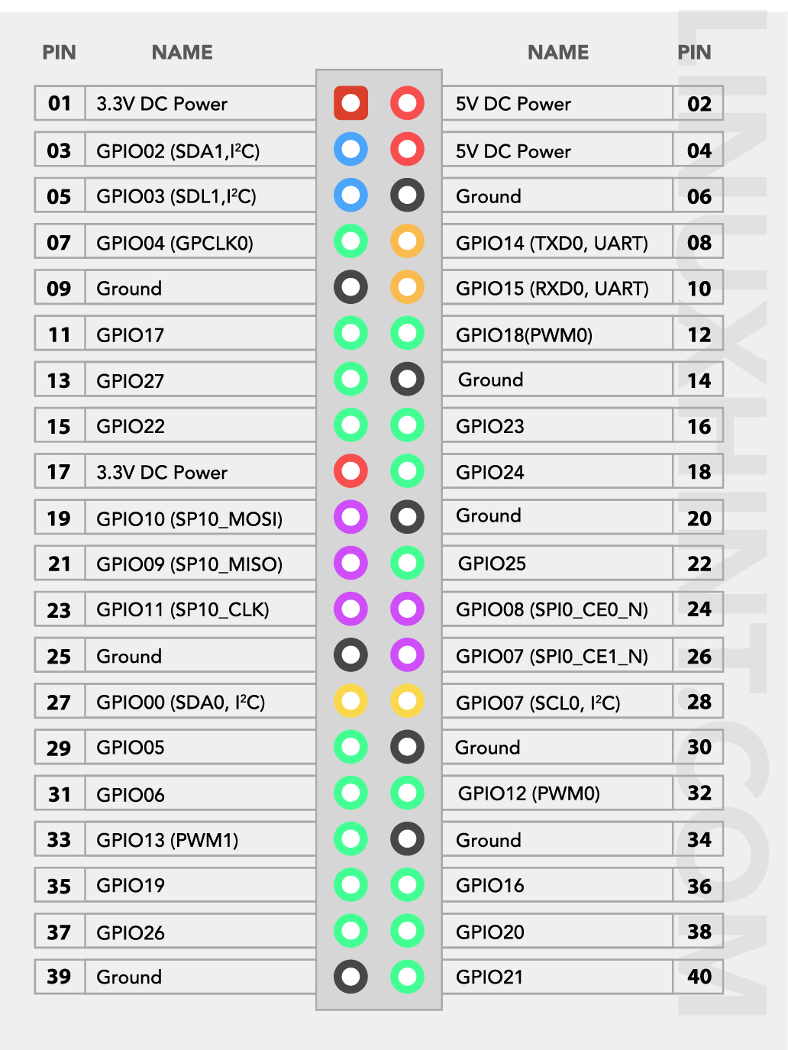
\includegraphics[width=0.4\textwidth]{obrazky/gpio_header.png}
    \caption{GPIO header Raspberry PI 4}
\end{figure}
\subsubsection{Komunikačné zbernice}
\section{Databáza}
Databáza (iné názvy: báza údajov, báza dát, dátová báza; zriedkavo: databanka, banka dát, banka údajov) je množina štruktúrovaných dát alebo informácií uložených v počítačovom systéme, takým spôsobom, že počítačový program alebo človek môže použiť dopytovací jazyk (napr. \acs{SQL}) na získavanie týchto informácií. Takto získané informácie môžu byť použité pri rozhodovacom procese. Počítačový program používaný na správu dát a tvorbu dopytov (queries) sa označuje SRBD (Systém riadenia bázy dát). Vlastnosťami a návrhom SRBD sa zaoberá informatika.
%wiki Databaza

\subsection{Príkazy \acl{DDL}}

\subsubsection{Prikaz Create}

\begin{lstlisting}[
           language=SQL,
           showspaces=false,
           basicstyle=\ttfamily,
           numbers=left,
           numberstyle=\tiny,
           commentstyle=\color{gray}           
        ]
CREATE TABLE table_name (
    column1 datatype,
    column2 datatype,
    column3 datatype,
   ....
);
\end{lstlisting}


\subsubsection{Príkaz Alter}
\begin{lstlisting}[
           language=SQL,
           showspaces=false,
           basicstyle=\ttfamily,
           numbers=left,
           numberstyle=\tiny,
           commentstyle=\color{gray}           
        ]
ALTER TABLE table_name
ADD column_name datatype;

\end{lstlisting}
\subsubsection{Príkaz Drop}
\begin{lstlisting}[
           language=SQL,
           showspaces=false,
           basicstyle=\ttfamily,
           numbers=left,
           numberstyle=\tiny,
           commentstyle=\color{gray}           
        ]
DROP TABLE table_name;

\end{lstlisting}

\subsection{Prikazy \acl{DML}}
\subsubsection{Príkaz Insert}

\begin{lstlisting}[
           language=SQL,
           showspaces=false,
           basicstyle=\ttfamily,
           numbers=left,
           numberstyle=\tiny,
           commentstyle=\color{gray}           
        ]
INSERT INTO table_name (column1, column2, column3, ...)
VALUES (value1, value2, value3, ...);

\end{lstlisting}

\subsubsection{Príkaz Delete}

\begin{lstlisting}[
           language=SQL,
           showspaces=false,
           basicstyle=\ttfamily,
           numbers=left,
           numberstyle=\tiny,
           commentstyle=\color{gray}           
        ]
DELETE FROM table_name WHERE condition;

\end{lstlisting}

\subsubsection{Prikaz Update}
\begin{lstlisting}[
           language=SQL,
           showspaces=false,
           basicstyle=\ttfamily,
           numbers=left,
           numberstyle=\tiny,
           commentstyle=\color{gray}           
        ]
UPDATE table_name
SET column1 = value1, column2 = value2, ...
WHERE condition;

\end{lstlisting}

\subsection{Príkaz Select}

\begin{lstlisting}[
           language=SQL,
           showspaces=false,
           basicstyle=\ttfamily,
           numbers=left,
           numberstyle=\tiny,
           commentstyle=\color{gray}           
        ]
SELECT column1, column2, ...
FROM table_name WHERE condition 
ORDER BY increasing GROUP BY column1 

\end{lstlisting}
\section{Python}
    \subsection{pouzite kniznice}
        \subsubsection{mail}
        \subsubsection{GPIO}
\section{Shell}
\section{Posielanie e-mailov}
\subsection{mime}
\subsection{smtp}
\section{php}
PHP bolo inšpirované jazykmi podporujúcimi procedurálne programovanie. Najviac vlastností prebralo od jazyka C a jazyka Perl. V neskorších verziách bolo rozšírené o možnosť používať objekty. Jedna zo zaujímavých vlastností PHP je, že umožňuje oveľa viac ako bežný skriptovací jazyk. Vďaka modulárnemu návrhu možno PHP používať aj na vývoj aplikácii s užívateľským rozhraním (GUI). PHP dokáže spolupracovať s relačnými databázami, ako napríklad MySQL, Oracle, IBM DB2, Microsoft SQL Server, PostgreSQL alebo SQLite, pričom si stále zachováva jednoduchú a priamočiaru syntax. PHP beží na takmer všetkých najrozšírenejších operačných systémoch, vrátane UNIXu, Linuxu, Windows či Mac OS X. Spolupracuje s najrozšírenejšími webovými servermi. Architektúra Linux-Apache-MySQL-PHP (zaužívaná skratka LAMP) a takisto Windows-Apache-MySQL-PHP (WAMP) sa stali veľmi obľúbenými v internetovom odvetví.
\section{\acl{UML}}
Unified Modeling Language alebo UML je v softvérovom inžinierstve grafický jazyk na vizualizáciu, špecifikáciu, navrhovanie a dokumentáciu programových systémov. UML ponúka štandardný spôsob zápisu tak návrhov systémov vrátane konceptuálnych prvkov ako sú business procesy a systémové funkcie, tak konkrétnych prvkov ako sú príkazy programovacieho jazyka, databázové schémy a znovupoužiteľné programové komponenty. UML podporuje objektovo orientovaný prístup k analýze, návrhu a popisu programových systémov. UML neobsahuje spôsob, ako sa má používať, ani neobsahuje metodiku, ako analyzovať, špecifikovať alebo navrhovať programové systémy. Štandard UML definuje štandardizačná skupina Object Management Group (OMG).
\subsection{Use Case diagramy}
\subsection{Diagramy aktivít}


